\documentclass[tikz,border=2pt]{standalone}
\usetikzlibrary{calc}
\usetikzlibrary{intersections}
\usetikzlibrary{patterns}
\usepackage{bm}
\usetikzlibrary{positioning}
\usetikzlibrary{shapes}
\usepackage{pgfplots}
\pgfplotsset{compat=1.18}

\begin{document}

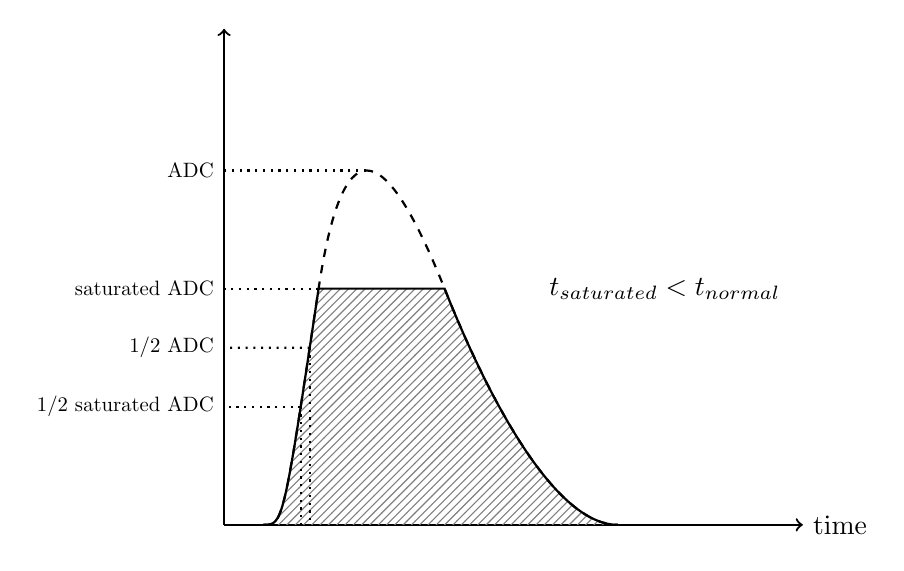
\begin{tikzpicture}[thick]

\pgfmathsetmacro{\xmin}{0}
\pgfmathsetmacro{\xmax}{7}
\pgfmathsetmacro{\deltax}{\xmax-\xmin}

\pgfmathsetmacro{\ymin}{0}
\pgfmathsetmacro{\ymax}{6}
\pgfmathsetmacro{\deltay}{\ymax-\ymin}

% % % --- Grille fine (repère) ---
% \draw[step=0.5cm, gray!30, very thin] (\xmin, \ymin) grid (\xmax,\ymax);
% % --- Grille épaisse tous les 1cm ---
% \draw[step=1cm, gray!60, thin] (\xmin, \ymin) grid (\xmax,\ymax);

% --- Axes ---
\draw[thick, ->] (\xmin,\ymin) -- (\xmax+0.05*\deltax,\ymin) node[right] {time};
\draw[thick, ->] (\xmin,\ymin) -- (\xmin,\ymax+0.05*\deltay);

% % --- Numérotation des axes ---
% \foreach \x in {\xmin,...,\xmax} {
%   \node[below] at (\x,0) {\footnotesize \x};
% }
% \foreach \y in {\ymin,...,\ymax} {
%   \node[left] at (0,\y) {\footnotesize \y};
% }
    
% \draw (0,0) -- (0.75,0) -- (1.5,5) -- (2,5) -- (4, 0) -- (6, 0);

% \draw [blue] (0.5,0) .. controls (0.75,0) .. (1.2,3);

% % pente descendente -2.5x + 10 = y so x = (10-y)/2.5
% \draw [red] (1.2,3) .. controls (1.5,5) and (2,5) .. (7/2.5,3);

% \draw [green] (7/2.5,3) .. controls (3,2.5) and (4,0) .. (5,0);

%%%%%%%%%%%%%%%%%%%%%%%%%%%%%%%%%%%%%%%%%%%%%%%%%%%%%%%%%%%%%%%%%%%%%%%%
% Uncomment the code above to see the construction procedure (you also need to comment the line below)
%%%%%%%%%%%%%%%%%%%%%%%%%%%%%%%%%%%%%%%%%%%%%%%%%%%%%%%%%%%%%%%%%%%%%%%%

% \draw [thin, gray, name path = saturatedPart, pattern=north east lines, pattern color=gray] (1.2,3)
%                      .. controls (1.5,5) and (2,5) .. (7/2.5,3) -- cycle; 



\draw [black, dashed, thick, name path = normalSignal] (0.5,0) .. controls (0.75,0) .. (1.2,3)
                     .. controls (1.5,5) and (2,5) .. (7/2.5,3)
                     .. controls (3,2.5) and (4,0) .. (5,0);

\draw [black, name path = saturatedSignal, pattern=north east lines, pattern color=gray] (0.5,0) .. controls (0.75,0) .. (1.2,3)
                     -- (7/2.5,3)
                     .. controls (3,2.5) and (4,0) .. (5,0);




% \draw [name path = normalThreshold, red] (0,2.25) -- (4, 2.25);
% \draw [name path = saturatedThreshold, red] (0,1.5) -- (4, 1.5);

\path [name path = normalThreshold, red] (0,2.25) -- (4, 2.25);
\path [name path = saturatedThreshold, red] (0,1.5) -- (4, 1.5);

\path [name intersections={of=normalSignal and normalThreshold, by={N1, N2}}];

\path [name intersections={of=normalSignal and saturatedThreshold, by={S1, S2}}];

% \filldraw (N1) circle [radius=1pt] node [above left] {\tiny N1};
% \filldraw (N2) circle [radius=1pt] node [above right] {\tiny N2};
% \filldraw (S1) circle [radius=1pt] node [above left] {\tiny S1};
% \filldraw (S2) circle [radius=1pt] node [above right] {\tiny S2};

% draw time
\draw [dotted] (N1) -- (N1 |- 0,0);
\draw [dotted] (S1) -- (S1 |- 0,0);

% \draw[thick, ->] (\xmin,\ymin) -- (\xmax+0.05*\deltax,\ymin) node[right] {$x$};
% \draw[thick, ->] (\xmin,\ymin) -- (\xmin,\ymax+0.05*\deltay) node[above] {$y$};

% draw ADC limits
\draw [dotted] (1.8,4.5) -- (0,4.5) node [left] {\scalebox{0.75}{ADC}};

\draw [dotted] (N1) -- (0,2.25) node [left] {\scalebox{0.75}{1/2 ADC}};

\draw [dotted] (1.2,3) -- (0,3) node [left] {\scalebox{0.75}{saturated ADC}};

\draw [dotted] (S1) -- (S1 -| 0,0) node [left] {\scalebox{0.75}{1/2 saturated ADC}};

\node [right] at (4,3) {$t_{saturated} < t_{normal}$};


\end{tikzpicture}


\end{document}